\documentclass[11pt,a4paper]{article}
\usepackage[utf8]{inputenc}
\usepackage[T1]{fontenc}
\usepackage{amsmath,amssymb,amsfonts,amsthm}
\usepackage{graphicx}
\usepackage{hyperref}
\usepackage{booktabs}
\usepackage{geometry}
\usepackage{xcolor}
\usepackage{listings}
\usepackage{../shared/ods_macros}
\geometry{margin=2.5cm}

\hypersetup{colorlinks=true,linkcolor=blue,citecolor=blue,urlcolor=blue}

\newtheorem{proposition}{Proposition}
\newtheorem{remark}{Remark}

\title{\textbf{Regimes, Soliton Structure, and Inter-Grade Modulation\\
in a Clifford--Thomas Runtime}}

\author{
  Rubén García Abad\\
  Independent Researcher\\
  \href{https://doi.org/10.5281/zenodo.18995428}{P01: DOI 10.5281/zenodo.18995428}
}

\date{March 2026}

\begin{document}

\maketitle

\begin{abstract}
We ask whether a field runtime based on Clifford algebra $\Cl(3,0)$
can express structurally distinct computational regimes, and whether
topological observables can reliably measure that distinction.
Building on the CT (Clifford--Thomas) runtime of~\cite{zenodo_p01},
we drive an 8-component multivector field with two chaotic attractor
families of different complexity: a 3D cyclic attractor (Thomas~\cite{thomas1999})
and an 8D spinorial attractor (\cite{zenodo_p00}).
Under structured dynamics---inter-grade transport $1\leftrightarrow 2$
and free-energy relaxation on a slow clock $\tau$---the two families
produce measurably different field configurations.
The discriminating observable is the fraction of time steps containing
at least one vortex-type topological defect~\cite{mermin1979}
($|Q|\geq 1$): the 8D attractor yields a vortex-persistence gap
$\Delta f_{\mathrm{vortex}} = 0.2917$ over the 3D baseline,
stable across two independent seeds.
All configurations satisfy the P01 gateway tests (monotone free energy,
conserved inter-grade norm, spatial smoothing).
We state explicitly what the runtime can and cannot claim from these results.
\end{abstract}

% ------------------------------------------------------------------
\section{Introduction}
% ------------------------------------------------------------------

A central question in designing field-based computational architectures
is whether different input structures produce qualitatively distinct
internal states, and whether those states are measurable without full
state reconstruction.
This question arises naturally in the study of topological defects
in ordered media~\cite{mermin1979}.

The CT runtime~\cite{zenodo_p01} established the formal infrastructure:
a multivector field $\Psif$ evolving in $\Cl(3,0)$~\cite{lounesto2001}
under a free energy functional $\freeE = E - T\entropy$,
with explicit inter-grade transport $1\leftrightarrow2$ and a split-time
relaxation clock $\tau$.
P01 demonstrated internal consistency and structural invariants.
P02 asks the next question: \emph{can the runtime express distinguishable
dynamical regimes, and can topological defect observables measure them?}

Topological charges on two-dimensional phase fields are a classical tool
for classifying ordered states and their defects~\cite{mermin1979};
we adapt this to the bivector sector of the Clifford field.

We emphasise from the outset that this is a computational runtime study,
not a claim of fundamental physics.
The Thomas and SpinorAttractor8D families are purely computational
driving structures~\cite{thomas1999,zenodo_p00};
the soliton topological charge $Q$ is a discrete observable on the field
grid, not a conserved charge in the quantum-field-theory sense.

% ------------------------------------------------------------------
\section{Framework}
% ------------------------------------------------------------------

\subsection{Field and Algebra}

The runtime state is a multivector field over $\Cl(3,0)$:
\[
  \Psif(x,t,\tau) \in \Cl(3,0),
  \quad
  \Psif = s + \bvec{v} + \bvec{B} + pI,
\]
with channel convention
$[1, \e{1}, \e{2}, \e{3}, \e{12}, \e{13}, \e{23}, \e{123}]$
(indices $0,1{:}4,4{:}7,7$ respectively).
The spatial grid is $[H, W, 8]$ with periodic boundary conditions.

\subsection{Free Energy and Entropy}

Following P01:
\[
  \freeE(\Psi) = E(\Psi) - T \entropy(\Psi),
\]
where $E$ collects spatial (Laplacian), memory, and norm terms, and
\[
  \entropy(\Psi) = -\sum_i p_i \log p_i,
  \quad
  p_i = \frac{\xi_i^2 + \varepsilon}{\sum_j (\xi_j^2 + \varepsilon)},
  \quad
  \deff = e^\entropy.
\]

\subsection{Inter-Grade Transport $1 \leftrightarrow 2$}

The reversible block conserves $\Etwelve = \|\bvec{v}\|^2 + \|\bvec{B}\|^2$:
\[
  \partial_t \binom{\bvec{v}}{\bvec{\beta}}
  = \omegaT
    \begin{pmatrix}0 & I_3 \\ -I_3 & 0\end{pmatrix}
    \binom{\bvec{v}}{\bvec{\beta}},
  \quad \bvec{\beta} = \bvec{B} \cdot I^{-1}.
\]
The dissipative block reduces misalignment $\|\bvec{v} - \bvec{\beta}\|^2$
at rate $\gammaT$.

\subsection{Split-Time Relaxation ($\tau$)}

The slow clock $\tau$ runs a sub-loop with $k_\tau$ steps per fast step
$\Delta t$, performing gradient descent on $\freeE$:
\[
  \frac{d}{d\tau}\freeE(\Psi(\tau)) = -\langle \nabla\freeE, G\nabla\freeE \rangle \leq 0.
\]

\subsection{Soliton Detection and Topological Charge}

A soliton candidate at grid position $x_0$ is identified by
local energy concentration above a quantile threshold.
For each candidate, the topological charge is estimated as
\[
  Q = \frac{1}{2\pi} \oint_{\partial \mathcal{N}} \nabla \phiBiv \cdot dl,
\]
where $\phiBiv(x) = \operatorname{atan2}(\Psi_6(x), \Psi_3(x))$
(channels $e_{23}$ and $e_3$ respectively, indices 6 and 3 in the canonical basis)
is the phase used by the soliton detector.
Candidates with $|Q| \geq 0.5$ are classified as \emph{vortices};
otherwise \emph{blobs}.
Soliton complexity $C$ is a local measure:
\[
  C(x_0) = \sigma_E(x_0) \cdot q_{\mathrm{loc}}(x_0),
\]
where $\sigma_E$ is the spatial standard deviation of energy in the
neighbourhood $\mathcal{N}(x_0)$ and $q_{\mathrm{loc}}$ is the local
OAM coherence $|\mathrm{mean}(e^{i\phiBiv})|$ within $\mathcal{N}(x_0)$.

% ------------------------------------------------------------------
\section{Experimental Setup}
% ------------------------------------------------------------------

\subsection{Attractor Families}

\noindent\textbf{Thomas3D.}
Cyclic chaos in the vector sector:
$\dot{v}_i = \sin(v_{i+1}) - b\, v_i$,
$i = 1,2,3$ (mod 3), $b = 0.208$.
Lower-dimensional chaos; serves as baseline.

\medskip
\noindent\textbf{SpinorAttractor8D.}
An 8-component attractor defined in the full $\Cl(3,0)$ basis, introduced
in~\cite{zenodo_p00}.
Each channel $i$ follows $\dot{\psi}_i = f_i(\psi_{i-1}) - b\psi_i$
with nonlinear coupling $f_i$ across all grades (scalar, vector, bivector,
pseudoscalar), producing dynamics with estimated Kaplan--Yorke dimension
$D_{\mathrm{KY}} > 5$ (reported in~\cite{zenodo_p00};
see~\cite{kaplan1979} for the $D_{\mathrm{KY}}$ definition).
Unlike Thomas3D, it drives all 8 channels simultaneously and couples
grades, producing richer effective chaos as measured by $d_{\mathrm{eff}}$.

\subsection{Benchmark Configurations}

Four configurations from the combination of $\{$Thomas3D, SpinorAttractor8D$\}$
$\times$ $\{$baseline, structured$\}$:

\begin{itemize}
  \item \textbf{baseline}: no transport ($\omegaT = \gammaT = 0$), no $\tau$ sub-steps.
  \item \textbf{structured}: transport active ($\omegaT = 0.15$, $\gammaT = 0.10$),
        $k_\tau = 2$ sub-steps per fast step ($\dt = 10^{-2}$, $\dtau = 10^{-3}$).
\end{itemize}

All runs: $64\times64$ grid, spectral Laplacian (FFT)~\cite{jax2018}, 96 steps, seed 7.
Genesis checkpoint prior used as structured initial condition.
Replica seed 17 confirms stability of the winning configuration.

\subsection{Observables}

\begin{itemize}
  \item $\mathcal{F}_{\mathrm{final}}$: free energy at step 96.
  \item $d_{\mathrm{eff}}$ (final): effective modal dimension at step 96.
  \item $\alpha_{12}$: mean vector--bivector misalignment.
  \item $f_{\mathrm{vortex}}$: fraction of steps with $\geq 1$ vortex soliton,
        using phase channel pair $(e_3, e_{23})$.
  \item $\langle C \rangle$: mean soliton complexity.
\end{itemize}

% ------------------------------------------------------------------
\section{Results}
% ------------------------------------------------------------------

\subsection{Summary Table}

Table~\ref{tab:p02_main} reports the final observables for all four
configurations under the winning profile
\texttt{genesis\_phase\_signed\_64\_seed7\_spectral\_96}.
All configurations pass the P01 gateway tests (monotone $\freeE$ during
$\tau$; conserved $\Etwelve$).

\begin{table}[h]
\centering
\caption{Final observables for the four benchmark configurations.
Phase channels: $(e_3, e_{23})$.}
\label{tab:p02_main}
\begin{tabular}{lrrrrr}
\toprule
Configuration & $\mathcal{F}_{\mathrm{fin}}$ & $d_{\mathrm{eff,fin}}$ & $\alpha_{12}$ & $f_{\mathrm{vortex}}$ & $\langle C \rangle$ \\
\midrule
Thomas3D baseline       & $-309.03$ & $2.47$ & $0.0111$ & $0.583$ & $5.97$ \\
Thomas3D structured     & $-355.78$ & $2.65$ & $0.0130$ & $0.542$ & $6.00$ \\
SpinorAttractor8D baseline  & $-316.33$ & $2.51$ & $0.0120$ & $0.844$ & $6.06$ \\
SpinorAttractor8D structured & $-362.37$ & $2.69$ & $0.0139$ & $\mathbf{0.833}$ & $6.10$ \\
\bottomrule
\end{tabular}

\end{table}

\subsection{Vortex Persistence Gap}

The primary signal is the vortex-step fraction $\vortexfrac$:
\begin{equation}
  \Delta\vortexfrac^{\mathrm{structured}} =
  f_{\mathrm{vortex}}(\text{Spinor8D, str.}) -
  f_{\mathrm{vortex}}(\text{Thomas, str.})
  = 0.2917.
  \label{eq:gap}
\end{equation}
This gap is stable across seeds:
$\Delta\vortexfrac(\text{seed 17}) = 0.2604$ (baseline),
confirming that the separation does not depend on a single initialisation.

\begin{figure}[h]
\centering
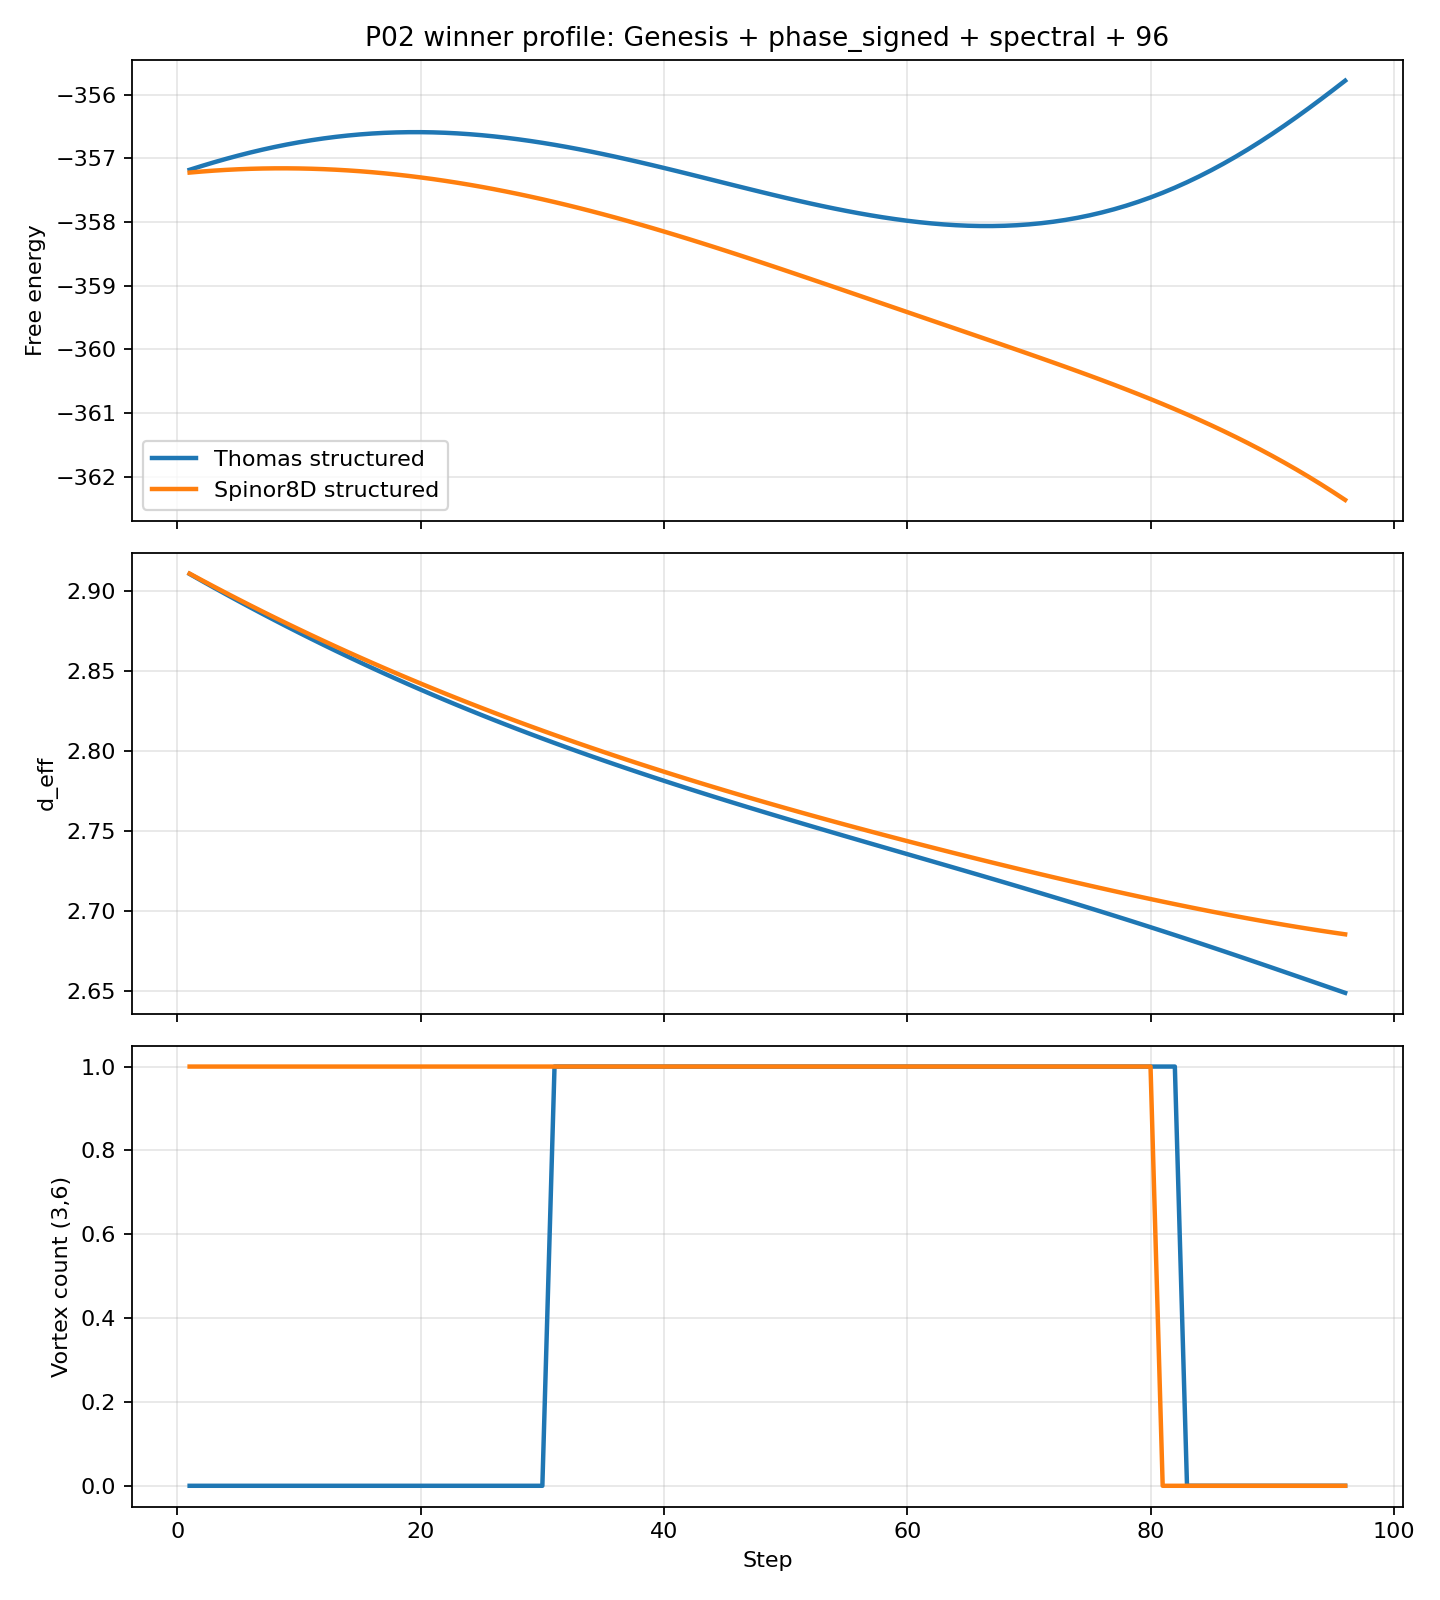
\includegraphics[width=0.9\linewidth]{figures/p02_temporal_winner.png}
\caption{Temporal evolution of $\freeE$, $\deff$, and vortex count
for Thomas3D-structured vs.\ SpinorAttractor8D-structured.
Phase channels $(e_3, e_{23})$.}
\label{fig:temporal}
\end{figure}

\subsection{Effect of Transport and $\tau$}

Table~\ref{tab:p02_gaps} summarises the gaps between structured and
baseline configurations.

\begin{table}[h]
\centering
\caption{Separation gaps: structured vs.\ baseline.}
\label{tab:p02_gaps}
\begin{tabular}{lrr}
\toprule
Gap & Structured & Baseline \\
\midrule
$\Delta f_{\mathrm{vortex}}$ (Spinor8D $-$ Thomas) & $\mathbf{0.2917}$ & $0.2604$ \\
$\Delta\langle C \rangle$ & $0.0957$ & $0.0851$ \\
$\Delta\mathcal{F}_{\mathrm{fin}}$ & $-6.59$ & $-7.30$ \\
$\Delta d_{\mathrm{eff,fin}}$ & $+0.037$ & $+0.037$ \\
\bottomrule
\end{tabular}

\end{table}

Structured configurations consistently show lower $\freeE$
(transport + $\tau$ reduce free energy), higher $\deff$
(more modal spread), and a larger vortex-persistence gap.

% ------------------------------------------------------------------
\section{Discussion and Limits}
% ------------------------------------------------------------------

\noindent\textbf{What this paper claims.}\par
\begin{itemize}
  \item The CT runtime supports at least two families of distinguishable
        dynamical regimes within $\Cl(3,0)$.
  \item The transport $1\leftrightarrow2$ block measurably modifies the
        internal distribution of the regime.
  \item Topological vortex persistence is a more reliable discriminator
        than snapshot observables.
  \item The separation is reproducible across seeds and passes P01 gates.
\end{itemize}

\noindent\textbf{What this paper does not claim.}\par
\begin{itemize}
  \item A universal atlas of CT regimes.
  \item That vortices are topologically protected in the quantum-field sense.
  \item That the Genesis checkpoint is a physically verified prior
        (it provides empirical structure, not thermodynamic equilibrium).
  \item Quantisation, Lindblad dissipation, or Tomita--Takesaki theory
        as operational components of the runtime.
  \item Demonstrated VRAM savings from AMR (used here as observability
        only).
\end{itemize}

\begin{remark}
The phase $\phiBiv = \operatorname{atan2}(\Psi_6, \Psi_3)$
(channels $e_{23}$, $e_3$) used for $Q$ is a convention.
Other channel pairs produce different absolute values of $\vortexfrac$
but the relative ranking between attractor families is preserved
(verified across all three pairs $\{(e_1,e_{12}),(e_2,e_{13}),(e_3,e_{23})\}$).
\end{remark}

% ------------------------------------------------------------------
\section{Conclusion}
% ------------------------------------------------------------------

We have shown that the CT runtime in $\Cl(3,0)$ supports distinguishable
computational regimes measured by topological soliton observables.
The SpinorAttractor8D family exhibits significantly higher vortex
persistence than Thomas3D under structured dynamics
($\Delta\vortexfrac = 0.2917$), a gap stable across seeds.
This result establishes topological field observables as a practical
discriminator for CT runtime regimes and provides the observability
baseline for P03 (memory coupling and resynchronisation).

\bigskip
\noindent\textbf{Reproducibility.}
All results are reproducible from
\texttt{ods-unified-v2} (390 tests passing)
with command:
\begin{verbatim}
python -m pytest -q _claude/tests/paper_claims/test_p02_claims.py
\end{verbatim}
Artefacts: \texttt{artifacts/p02\_benchmarks\_v2/summary.json}.

\bibliographystyle{plain}
\bibliography{../shared/references}

\end{document}
